\section{Datensatz}
\label{sec:02_Datensatz}

Der Datensatz wurde mittels einer PiCamera in einem Zeitraum von 3 Wochen
aufgenommen. 
Die Größe des Datensatzes ist beliebig erweiterbar aber wurde aufgrund der
zeitlichen Einschränkung zur Evaluation auf \num{4000} Fotos beschränkt. 

\begin{wrapfigure}{l}{0.35\textwidth}
		\centering
		\vspace{-0.5cm}
		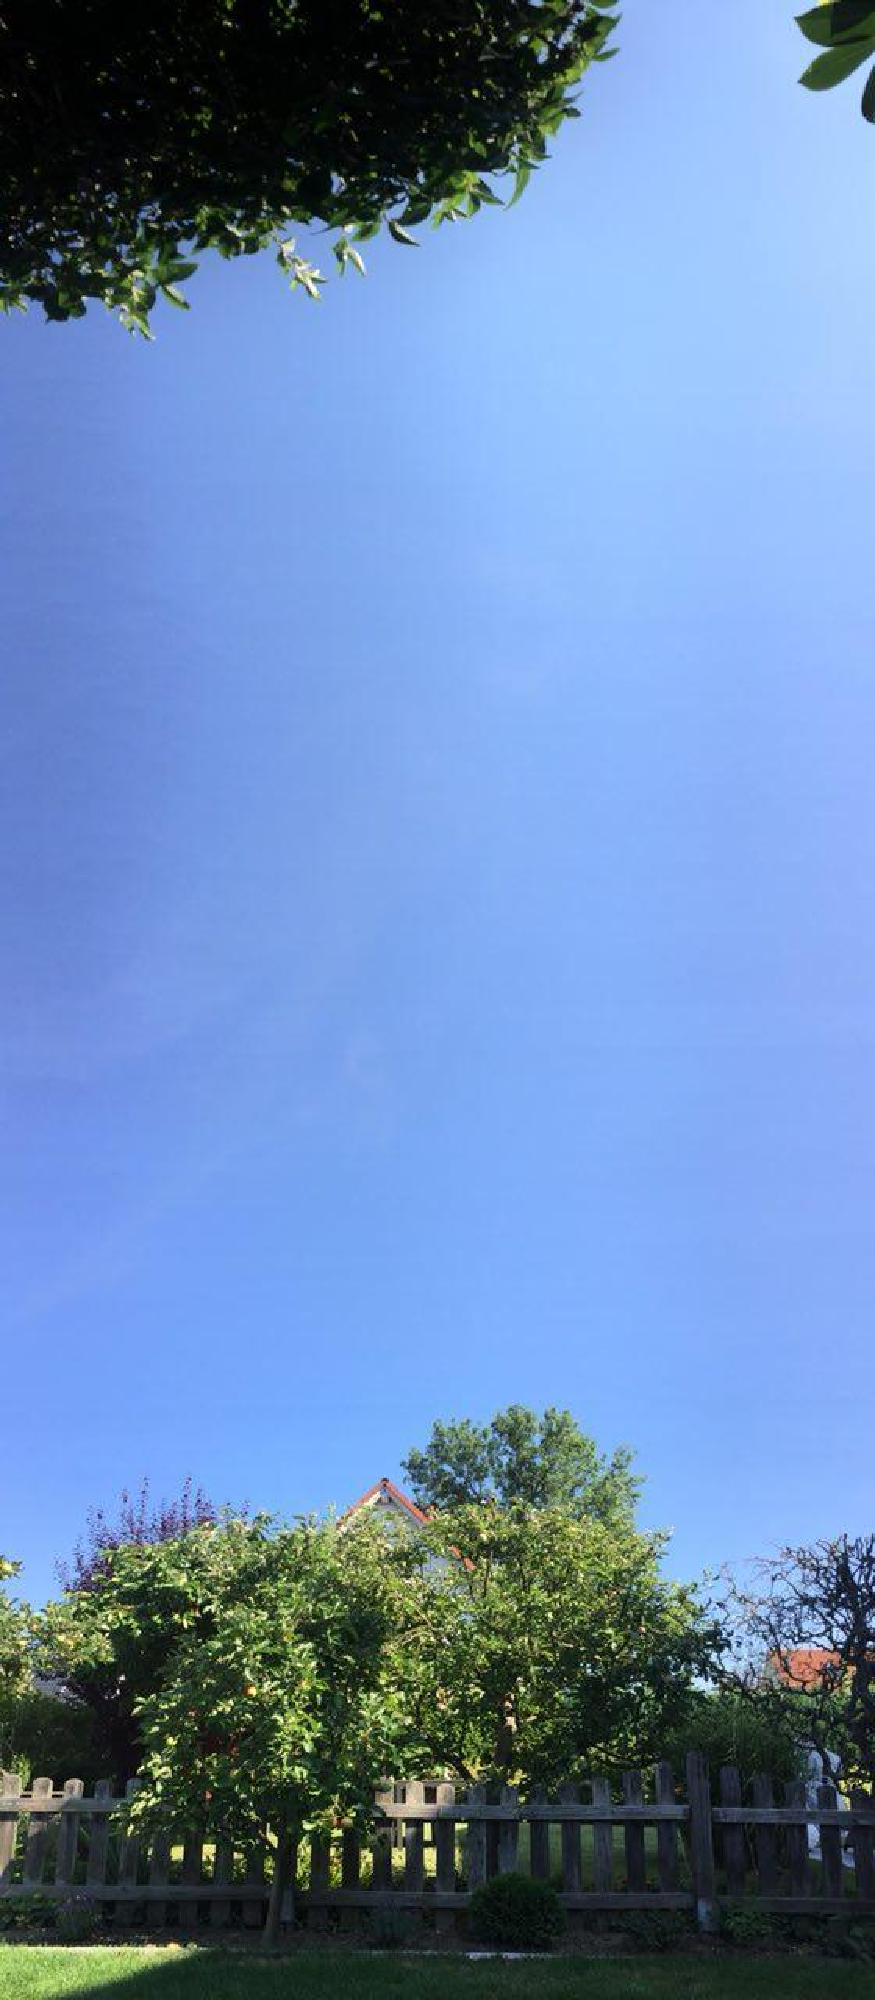
\includegraphics[width=0.3\textwidth]{./build/station_winkel.pdf}
		\caption{Wolkenausschnitt in Abhängigkeit des Observationswinkel}
		\label{fig:theta}
		\vspace{-0.5cm}
\end{wrapfigure}
Desweiteren spielt die Zeit in der die Daten aufgenommen werden eine 
wesentliche Rolle.
In Abhängigkeit mit der Jahreszeiten ändert sich die relativen Häufigkeit in 
der die verschiedene Wolkentypen aufgenommen werden können und somit in dem 
Datensatz repräsentiert sind. 
So sind zum Beispiel momentan (\today) Schönwetterwolken viel stärker vertreten
als die von Regenwetter. 
Zu den elf Wolkenklassen die auch die Klasse \textit{keine Wolken} einschließt 
zählt ebenso eine \textit{schlechtes Foto} Klasse. 
Aufgrund von zufälligen als auch zeitlichen Ereignissen werden Fotos produziert
die nicht Klassifiziert werden können.
Dies ist Beispielsweise der Fall, wenn eine Person das Sichtfeld verdeckt oder 
aufgrund der fehlenden Belichtung bei Nacht die Wolkendecke nicht erkannt wird.

Die Wolkenfotos wurden an zwei voneinander unabhängigen Orten aufgenommen, wobei
Charakteristiken der Aufnahmeorte auf den Bildern zu erkennen seien können.
Desweiteren stellte sich bei der Aufnahme des Datensatzes heraus, dass eine
Ausrichtung der Kamera der Wetterstation nach Norden sinnvoll ist.
Dadurch lässt sich der Kamerasensor schonen, indem ein übermäßiges ausleuchten
 des Bildes durch die Sonne verhindert wird.

Durch die Ausrichtung der Kamera zum Horizont kann, wie in Abbildung
 \ref{fig:theta} dargestellt, die Größe der observierten Wolken Fläche 
eingestellt werden.
Dadurch das die Wolken bei großen Aufnahmewinkeln $\theta$ viel näher als bei
kleinen $\theta$ sind, kann bei gleichbleibender Raumwinkelauflösung $\Omega$
nur eine viel kleinere Teil der Wolkendecke observiert werden.
Bei diesen Ausschnitten stellt es sich als schwierig heraus sie der richtigen
Klasse zuzuordnen da der Ausschnitt meist mehreren Klassen zuzuordnen ist. 

\begin{wrapfigure}{r}{0.35\textwidth}
		\vspace{-1.4cm}
		\centering
		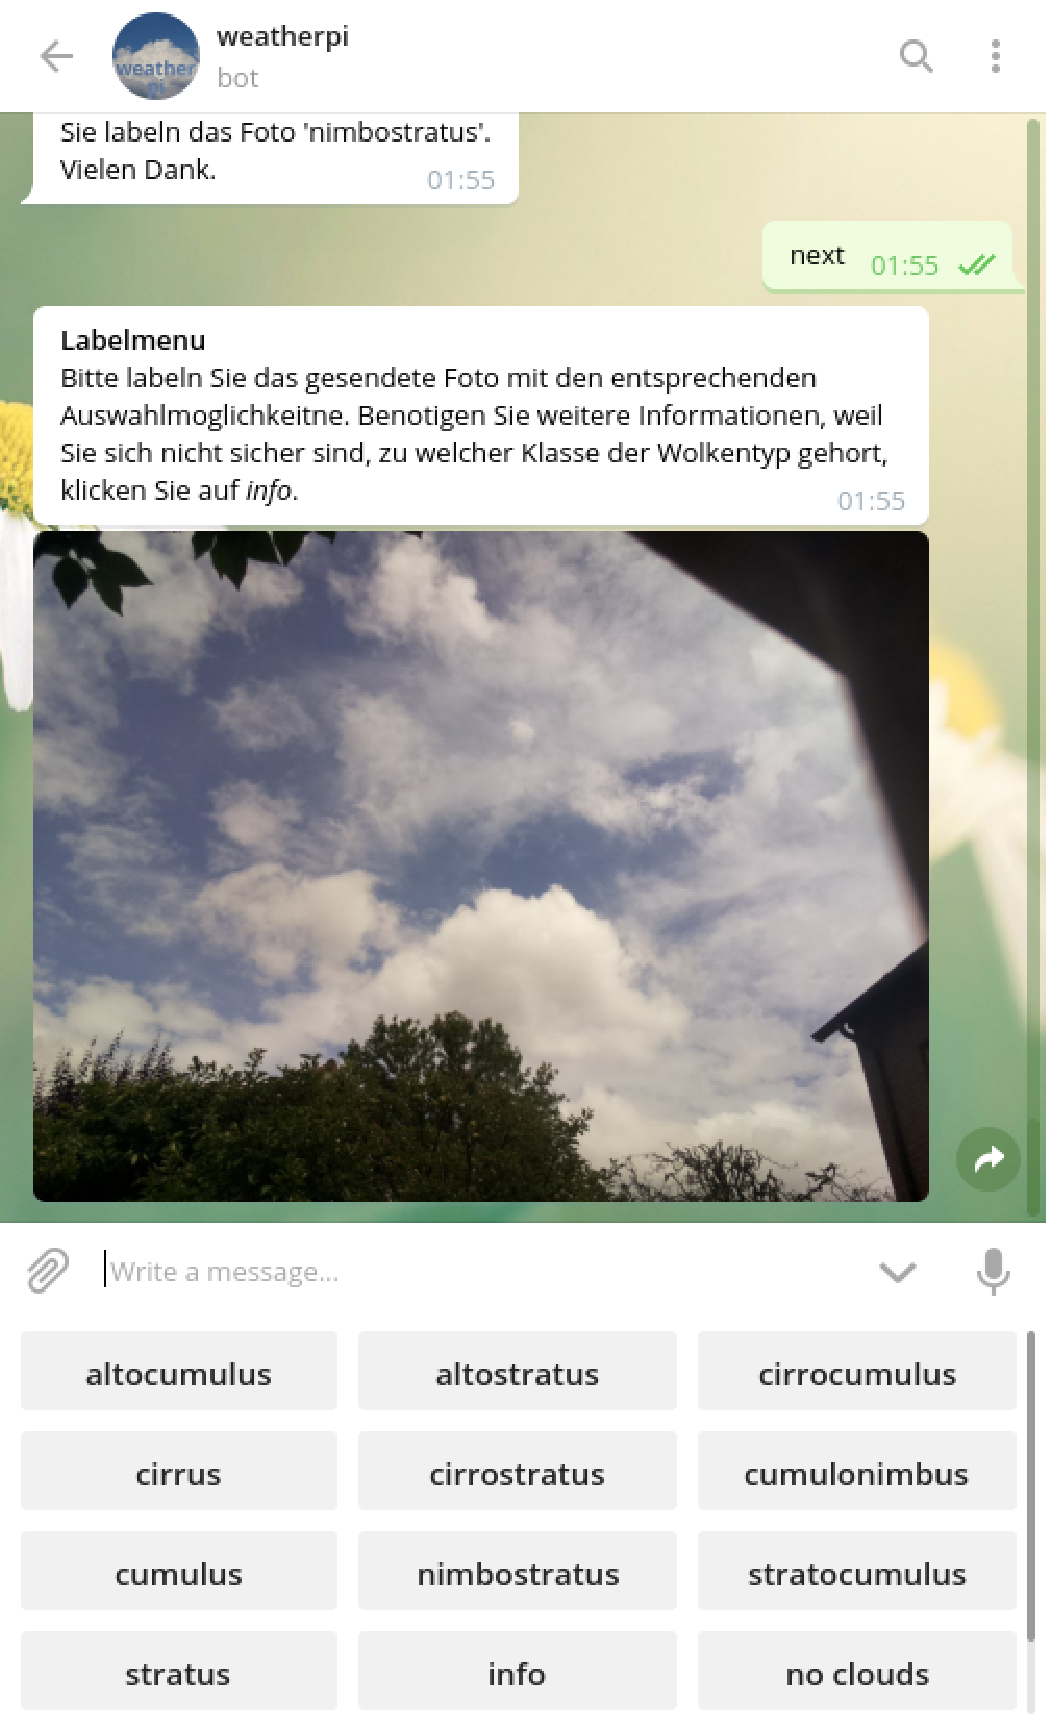
\includegraphics[width=0.35\textwidth]{pictures/telegram.pdf}
		\caption{\href{https://telegram.me/weatherpi_bot}{\texttt{TelegramBot}} zum Labeln der Wolkenfotos.}
		\label{fig:}
		\vspace{-1.0cm}
\end{wrapfigure}
Die aufgenommenen Daten besitzen a priori kein Label und sind auch nicht immer
eindeutig einer Klasse zuzuordnen.
Die Wolkenfotos wurden mittels eines eigen dafür programmierten
\href{https://telegram.me/weatherpi_bot}{\texttt{TelegramBot}} in
die in Abbildung~\ref{fig:classes} aufgeführten Kategorien eingeteilt.
Mit Hilfe von freiwilligen Labelern wurde jedes Foto des Datensatzes drei mal
klassifiziert und anschließend per Mehrheitsentscheidung der Zielklasse 
zugeteilt.
Der Arbeitsaufwand wurde mit ca $\num{4000} \, \text{Bilder} \cdot \SI{1}{\hertz}$
abgeschätzt.
Aufgrund von Aussetzern des Bots als auch der Ladezeiten der Bilder konnte die Rate
auch nach einer Einarbeitungszeit nicht erreicht werden und die pro Bild benötigte Zeit entsprach schätzungsweise
\SI{15}{\second}.
Bei der Evaluation der Modelle stellte sich heraus das bei paralleler Nutzung
eine interne Klassenvariable überschrieben wurde, sodass ein Großteil der
Klassifizierten Daten einer falschen Finalen Klasse zugeordnet wurden. 
Final steht ein Datensatz von \num{4000} Bildern welche in 10 Wolkenklassen und
einer Klasse mit schlechten Fotos aufgeteilt sind. Die Bilder besitzen eine Dimension 
von \texttt{(1024x768x3)} und liegen im \texttt{JPG}-Format vor.
Sie stehen unter der MIT Liezens und soll allen interessierten 
Datenanalysen zur Verfügung stehen.

\begin{figure}[h]
		\centering
		\begin{subfigure}[b]{0.31\textwidth}
		\begin{center}
				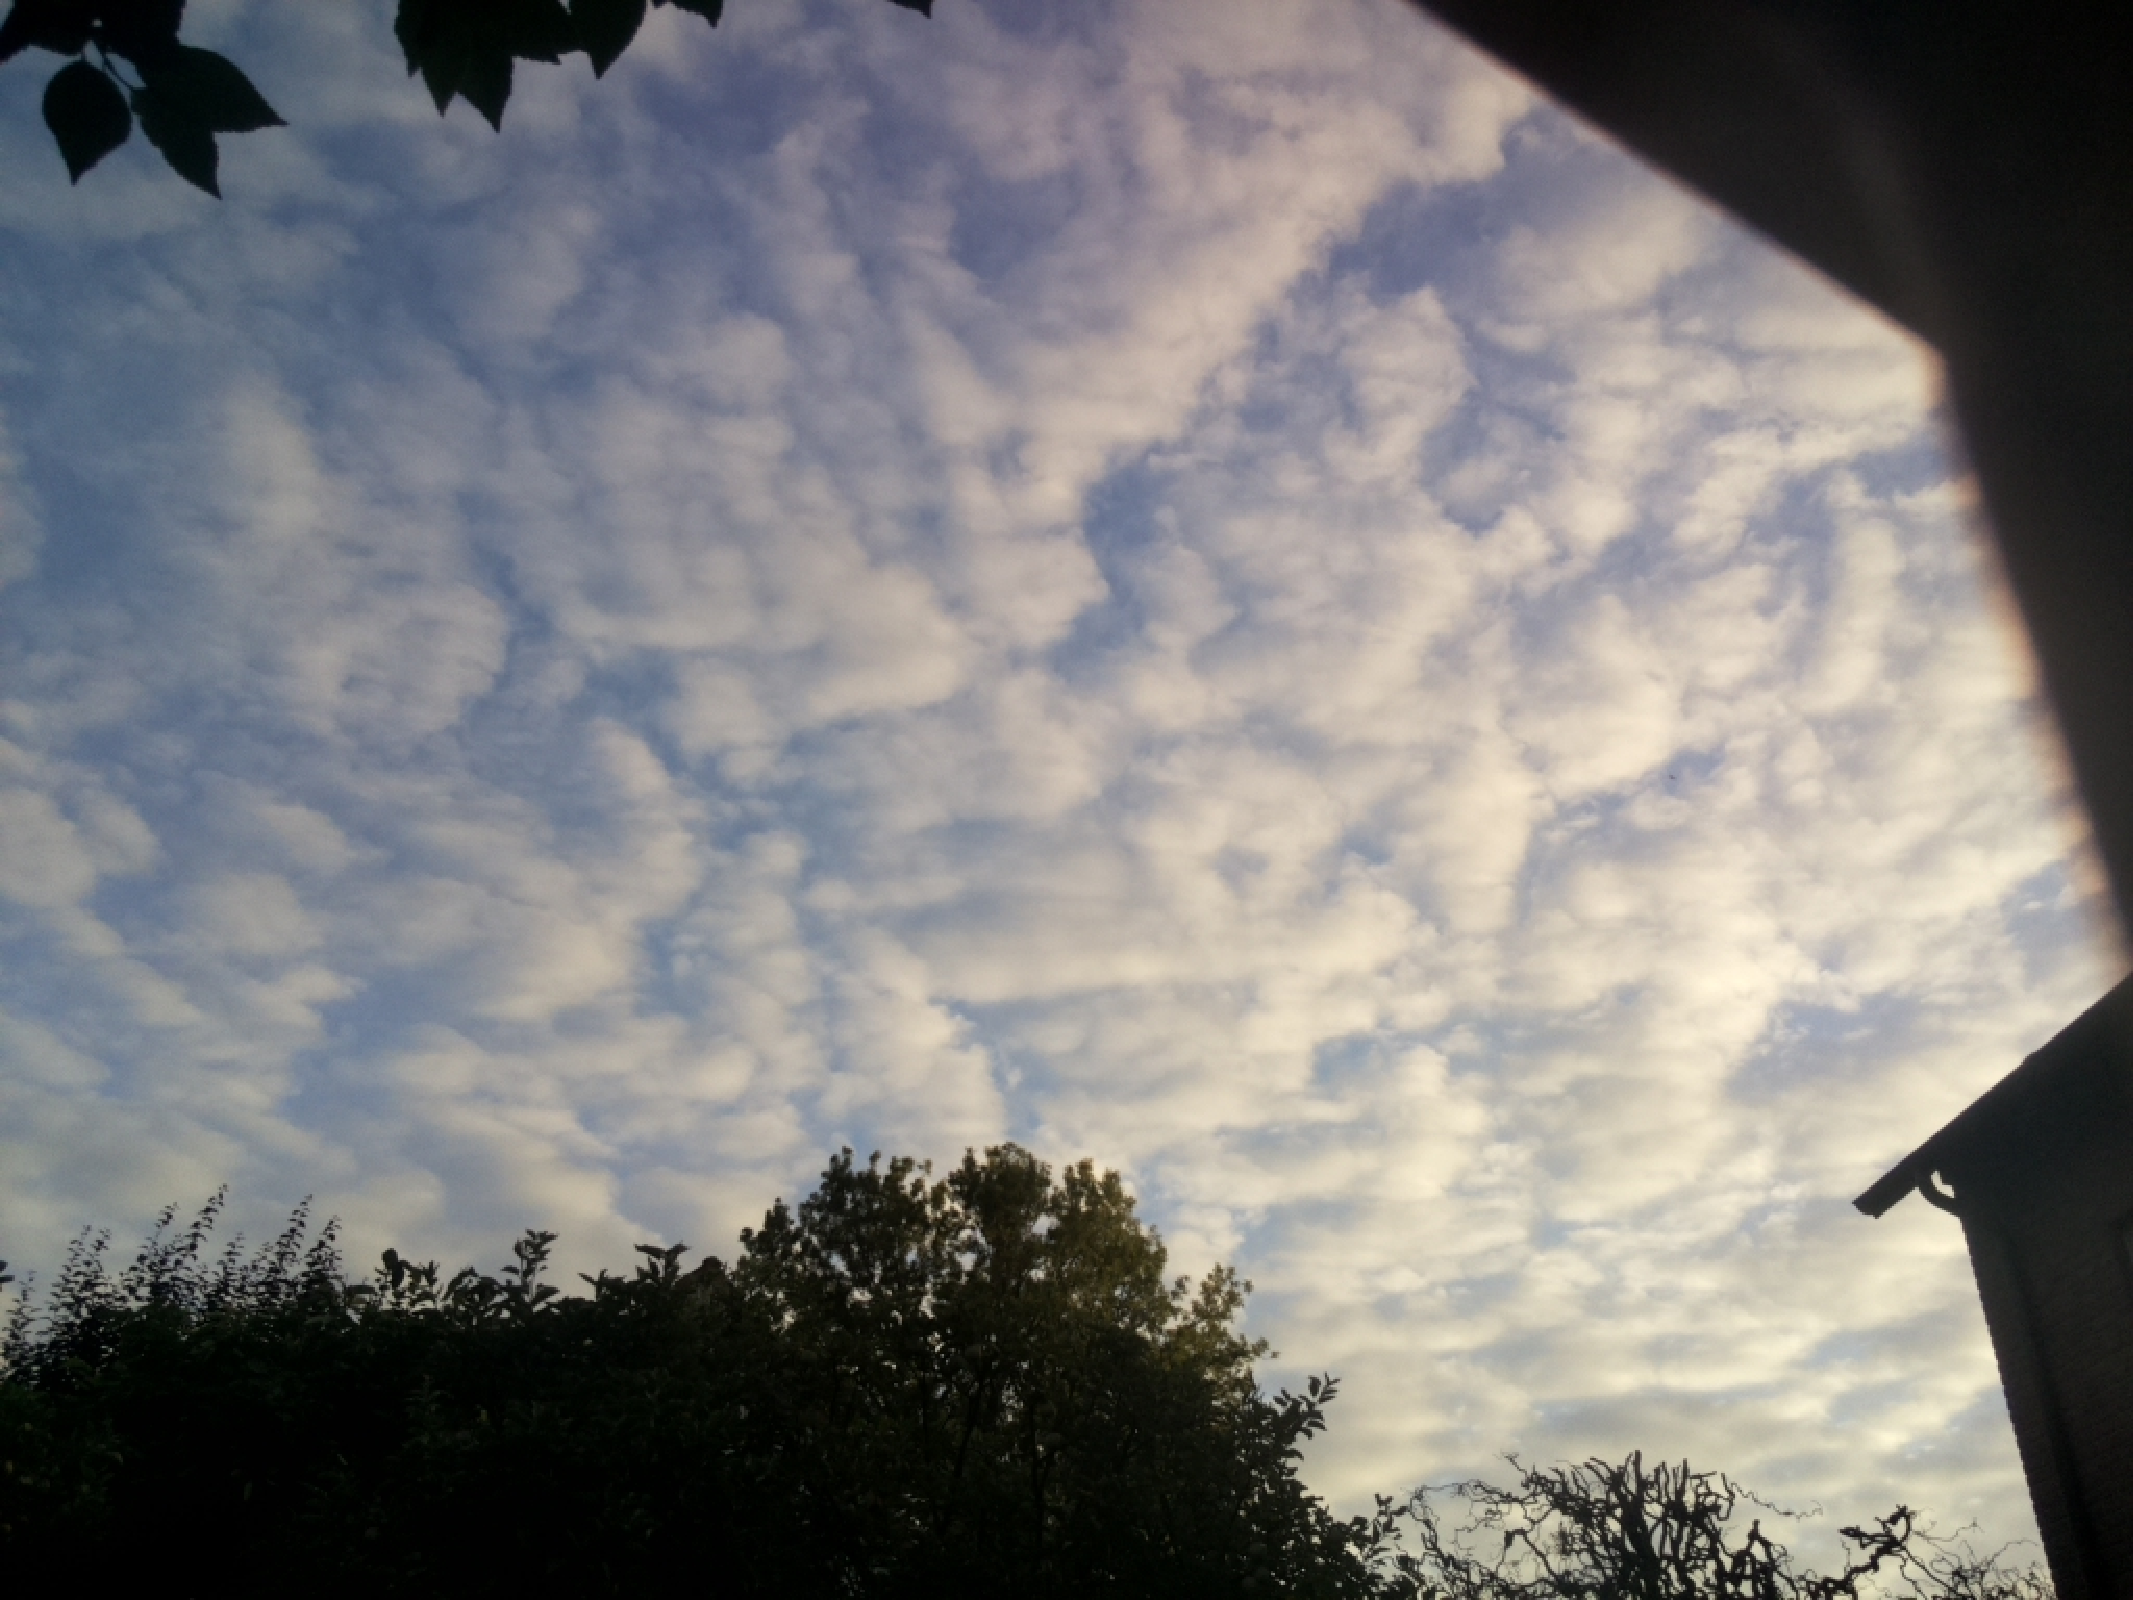
\includegraphics[width=\textwidth]{./pictures/cloudtypes/altocumulus.pdf}
		\end{center}
		\caption{Altocumulus}
		\label{fig:altostratus}
		\end{subfigure}
		\begin{subfigure}[b]{0.31\textwidth}
		\begin{center}
				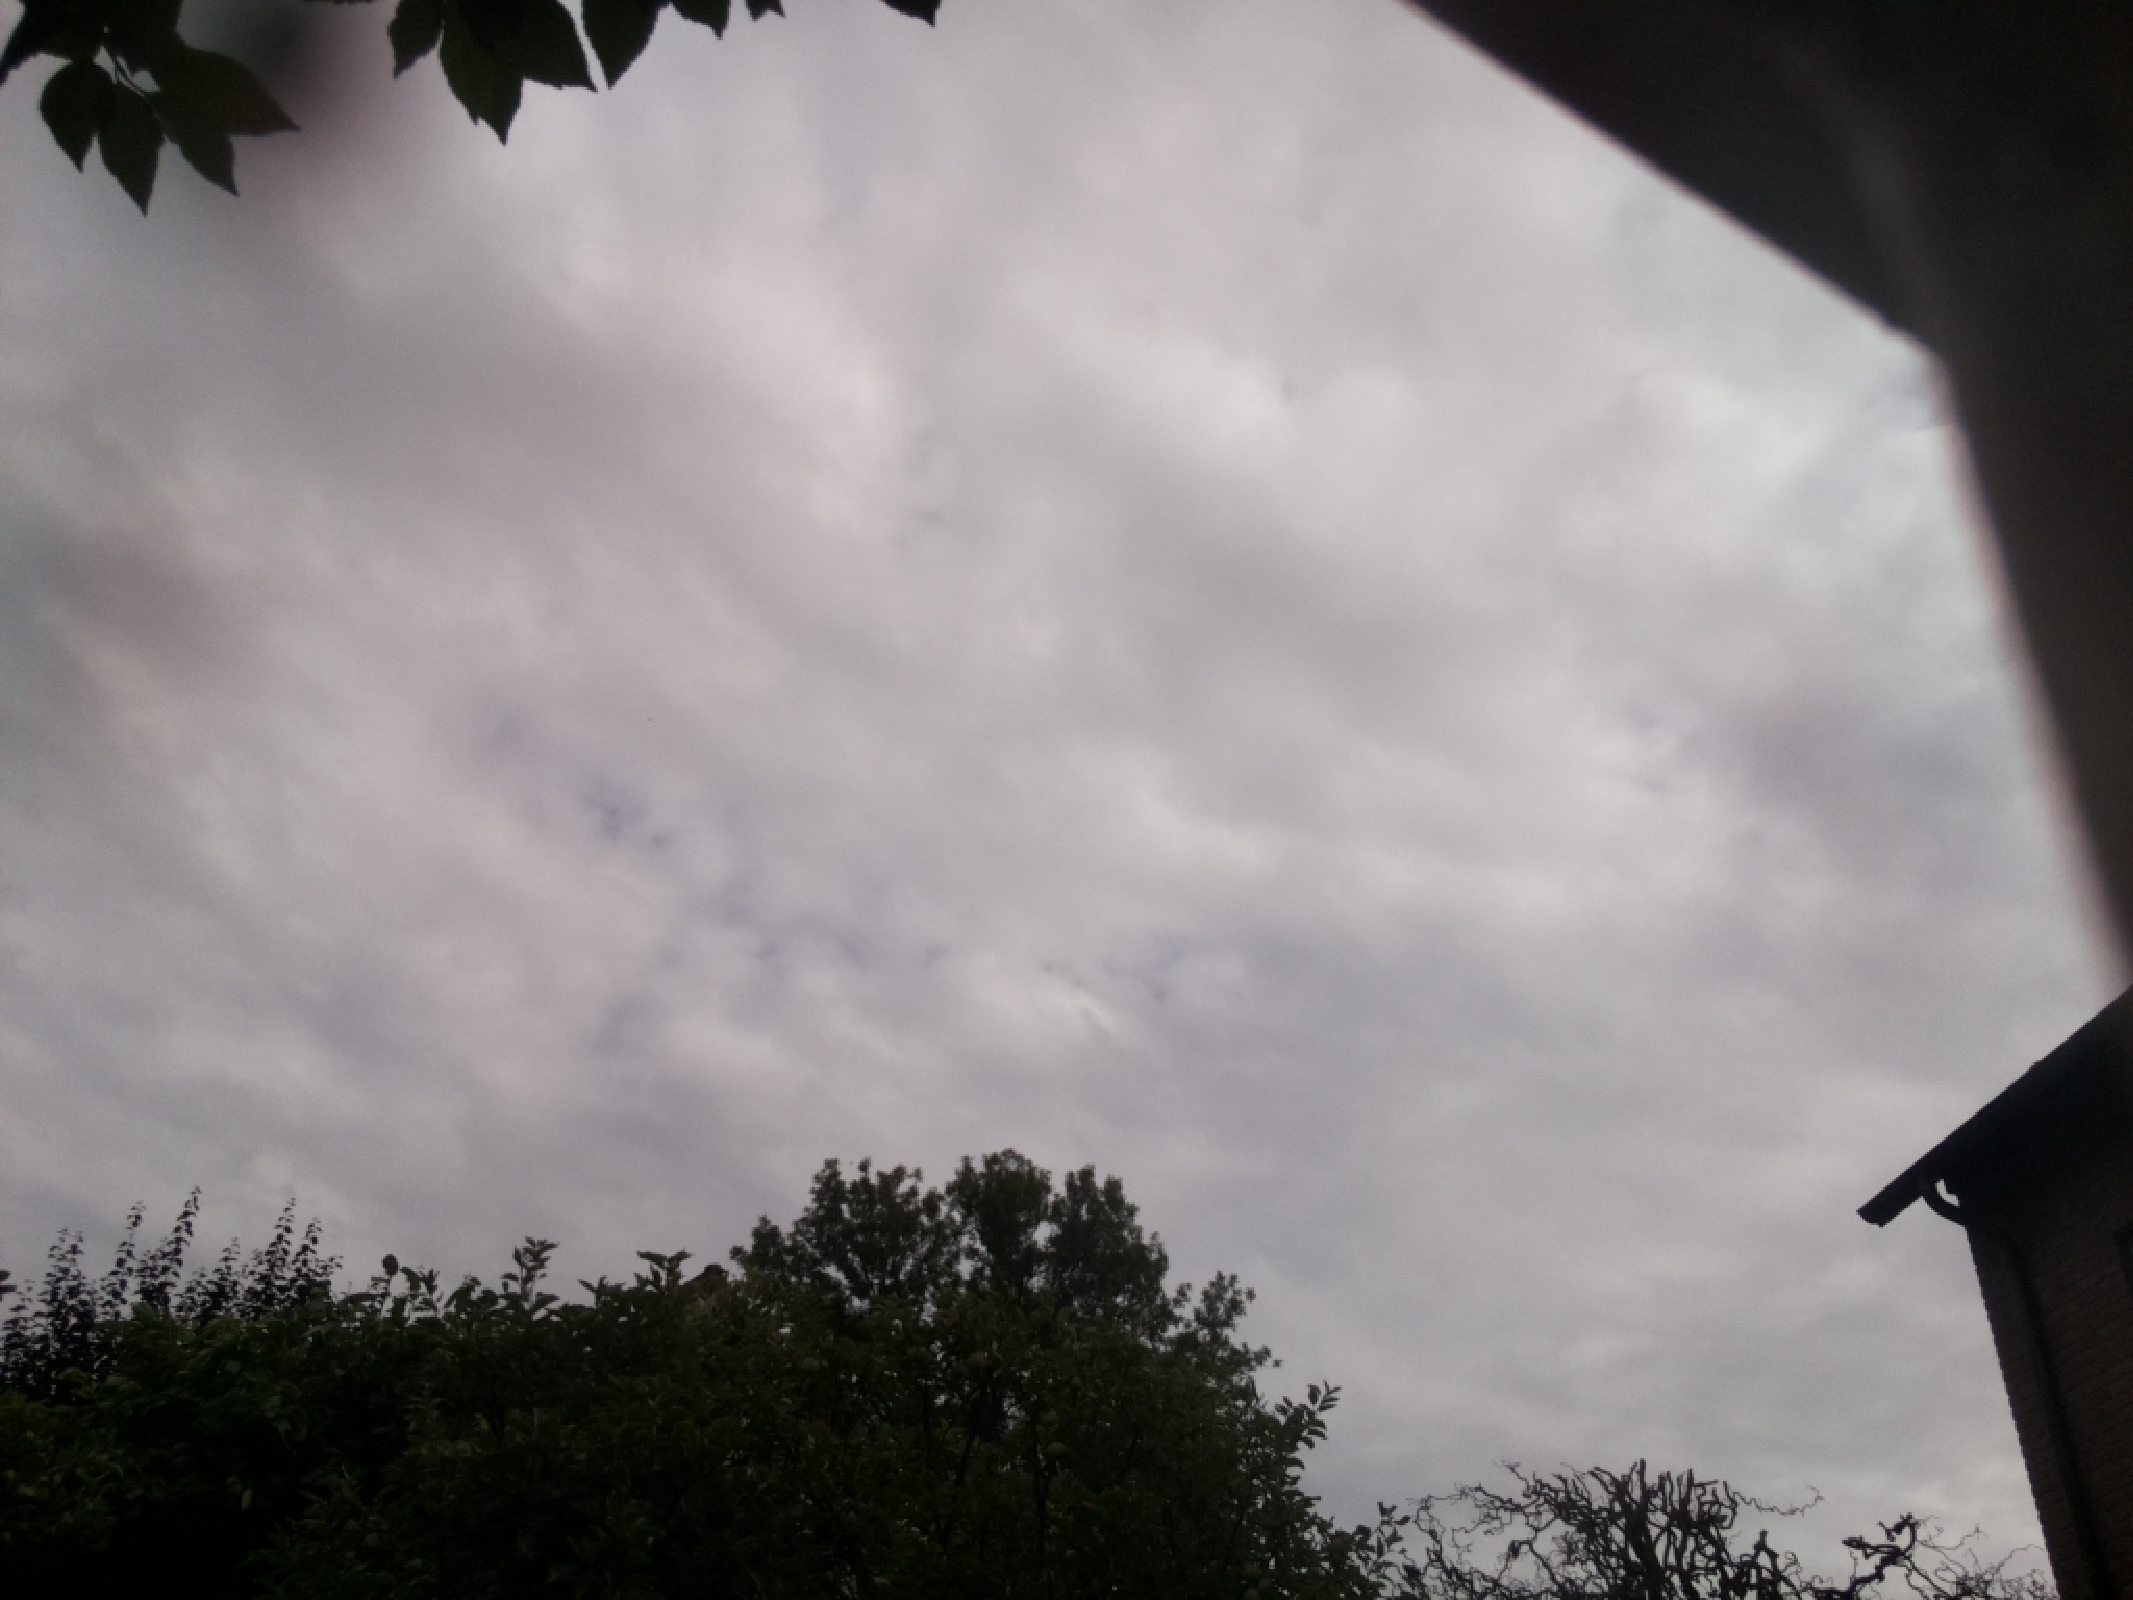
\includegraphics[width=\textwidth]{./pictures/cloudtypes/altostratus.pdf}
		\end{center}
		\caption{Altostratus}
		\label{fig:altocumulus}
		\end{subfigure}
		\begin{subfigure}[b]{0.31\textwidth}
		\begin{center}
				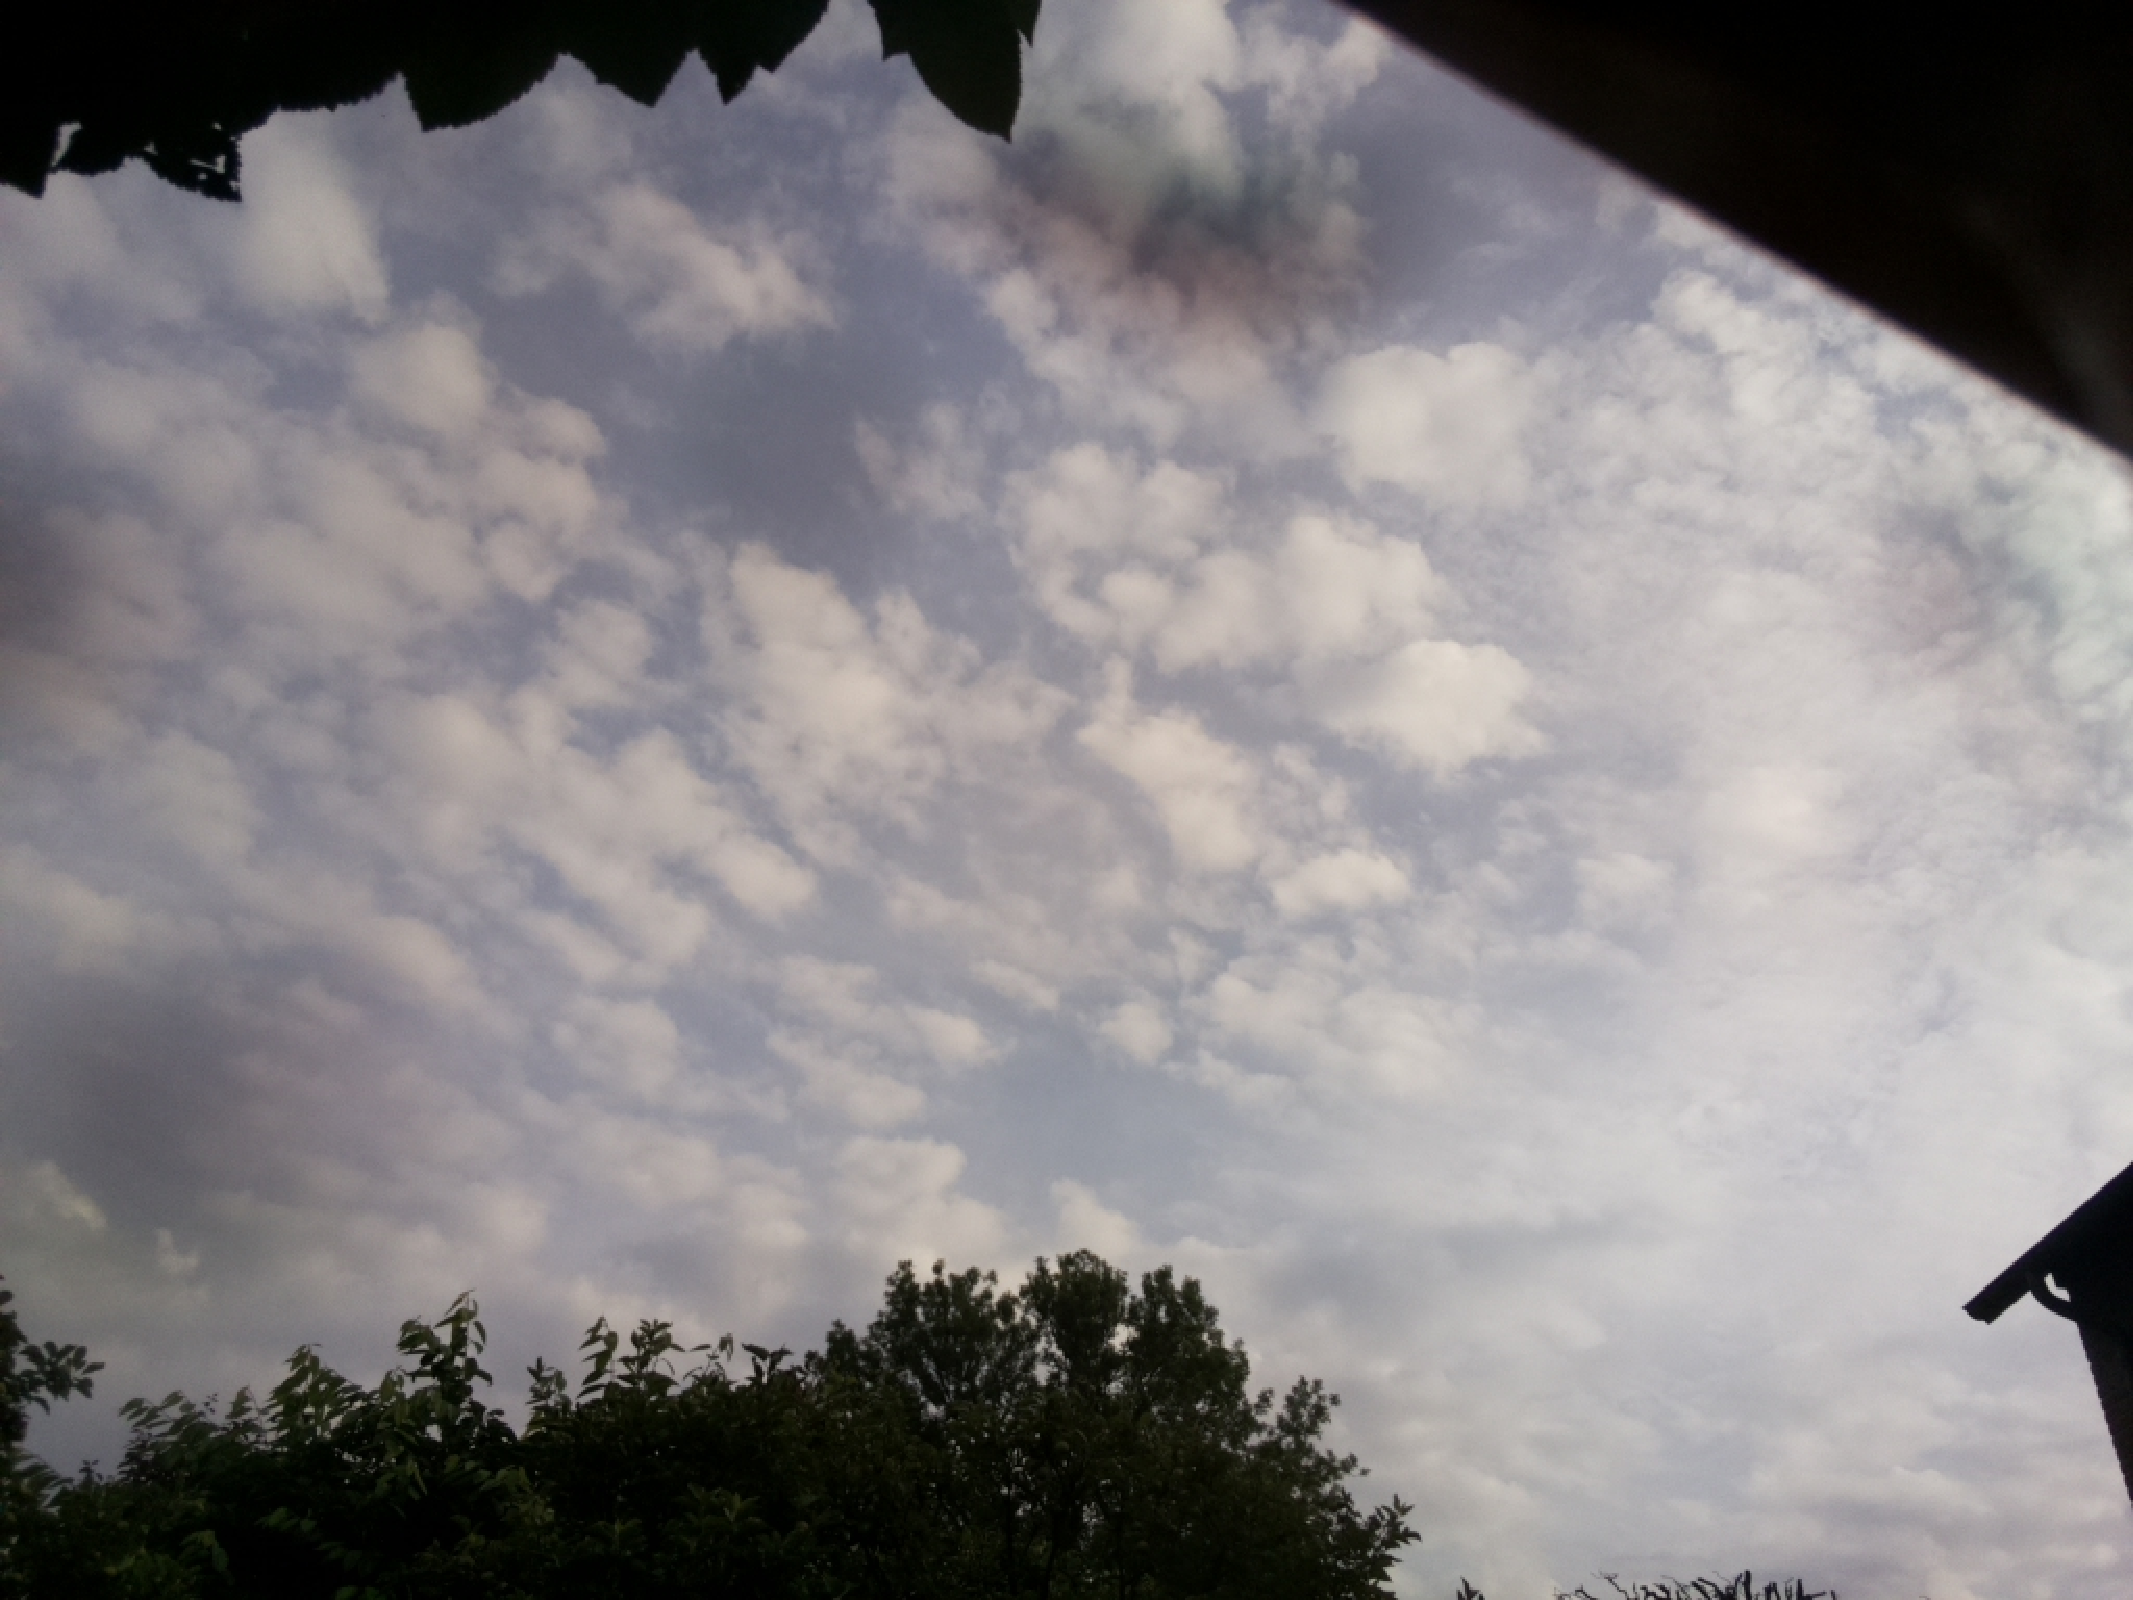
\includegraphics[width=\textwidth]{./pictures/cloudtypes/cirrocumulus.pdf}
		\end{center}
		\caption{Cirrocumulus}
		\label{fig:cirrocumulus}
		\end{subfigure}
		\begin{subfigure}[b]{0.31\textwidth}
		\begin{center}
				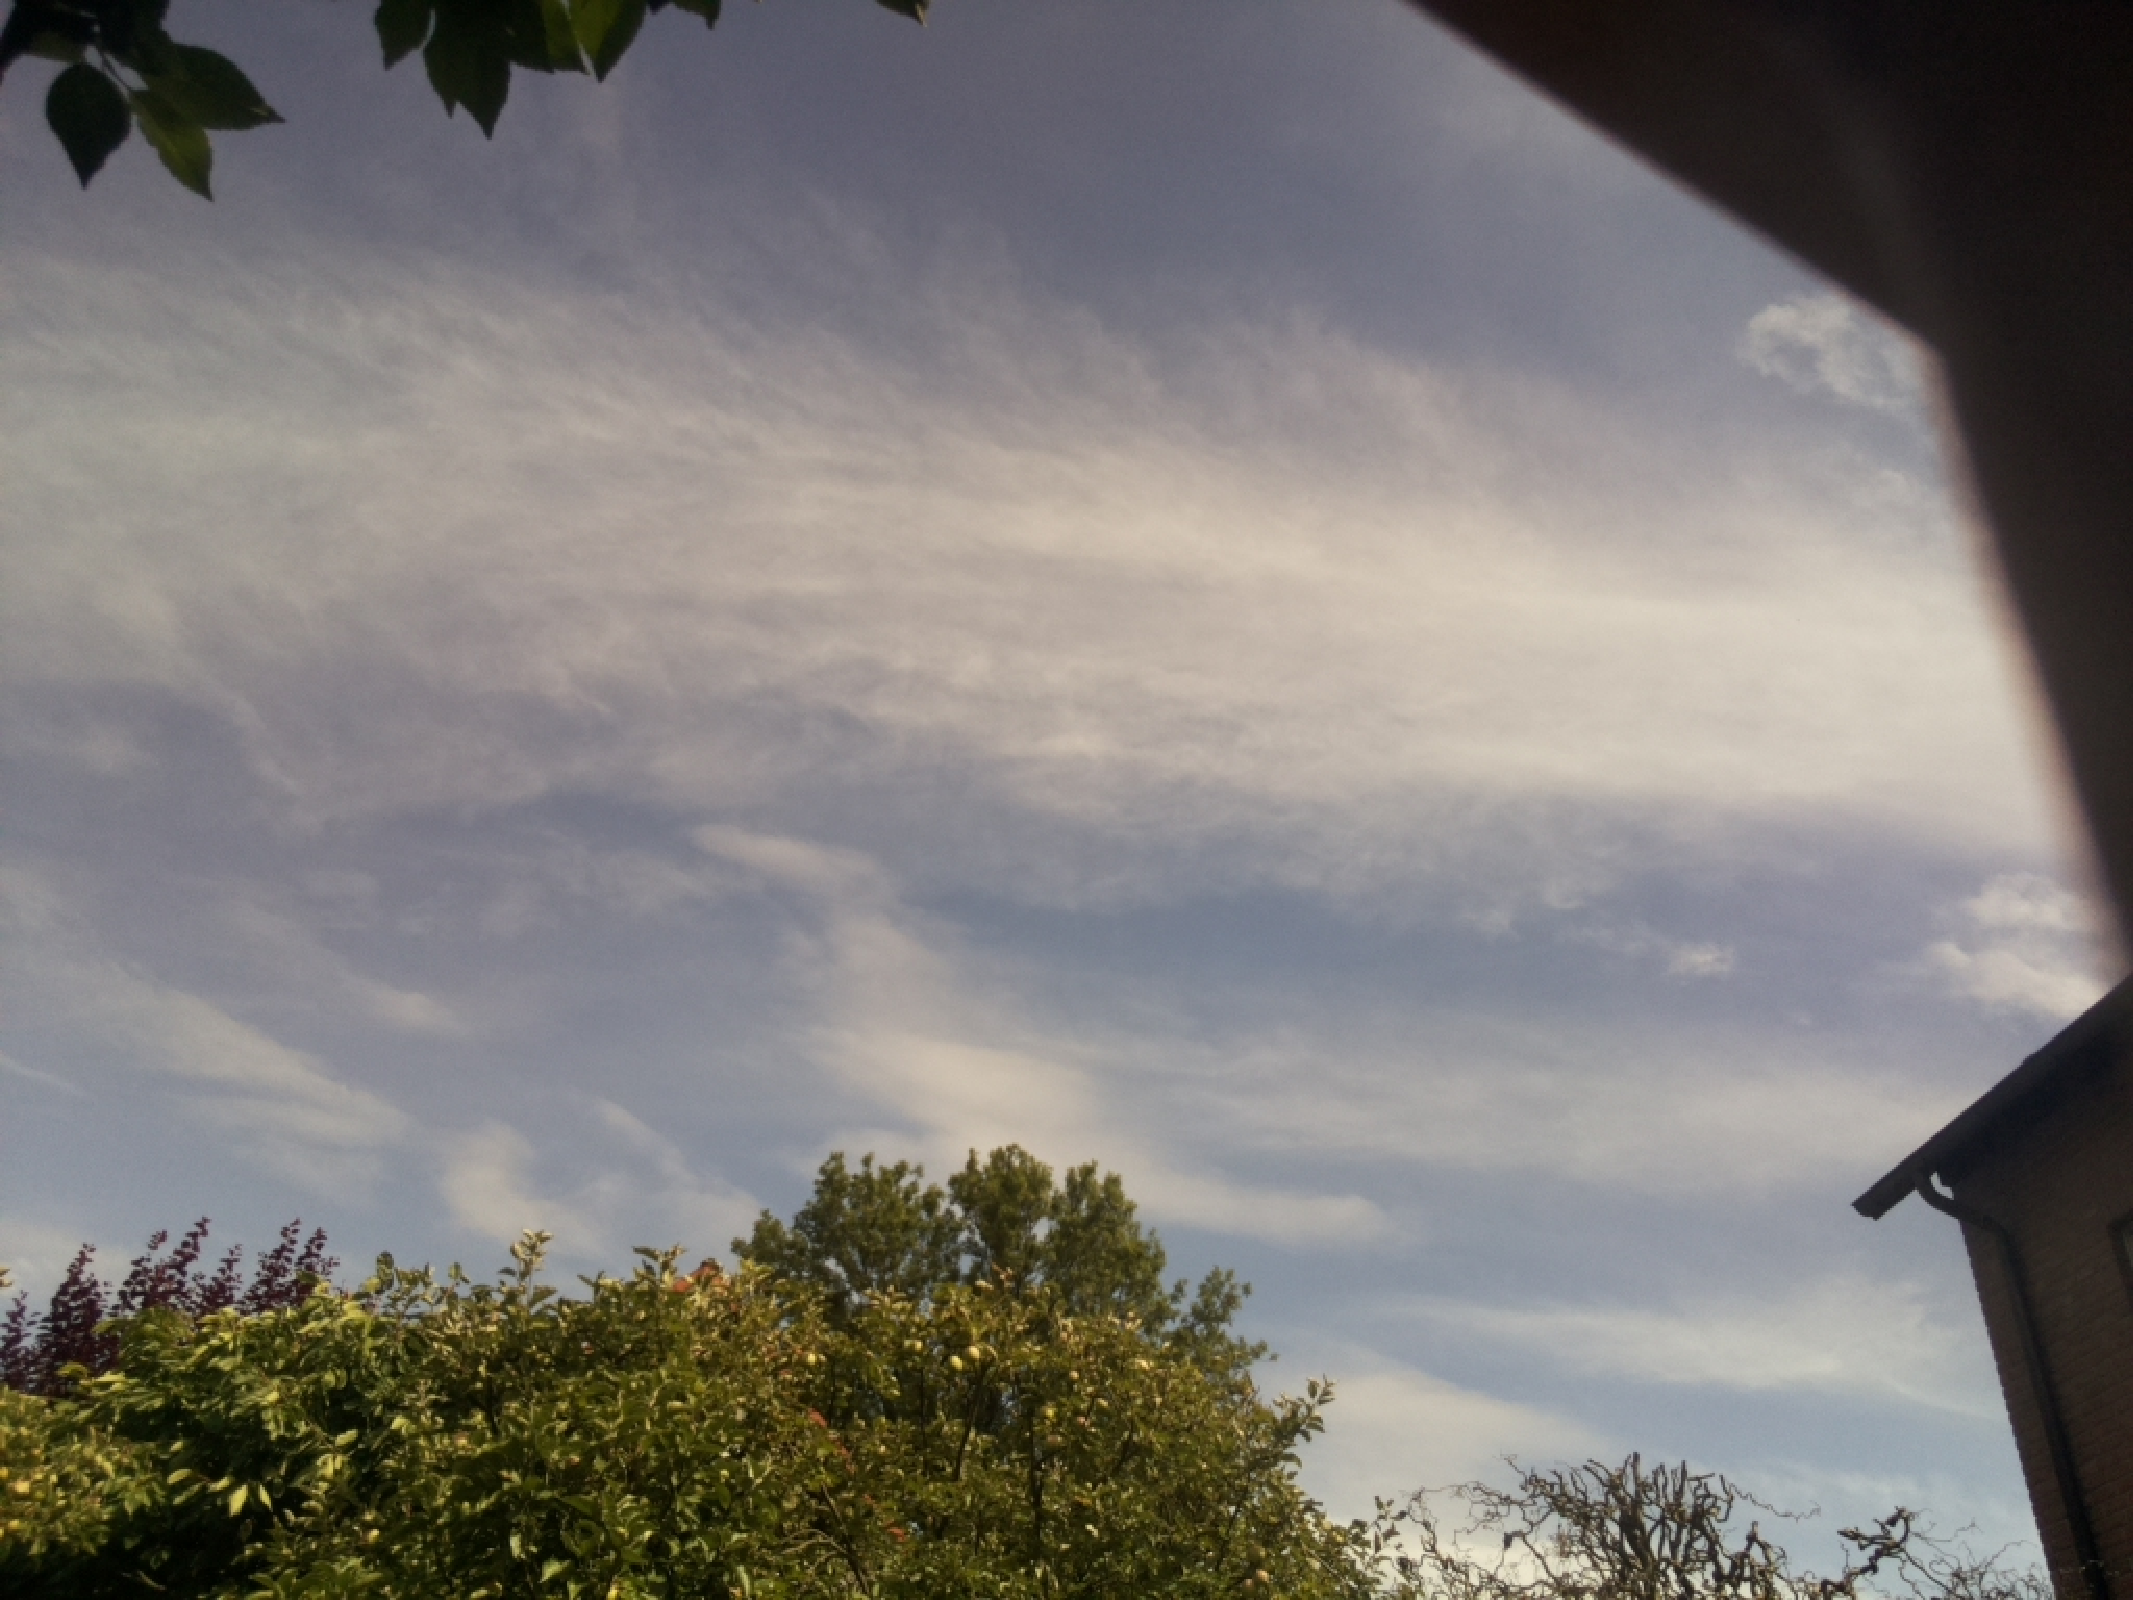
\includegraphics[width=\textwidth]{./pictures/cloudtypes/cirrostratus.pdf}
		\end{center}
		\caption{Cirrostratus}
		\label{fig:cirrostratus}
		\end{subfigure}
		\begin{subfigure}[b]{0.31\textwidth}
		\begin{center}
				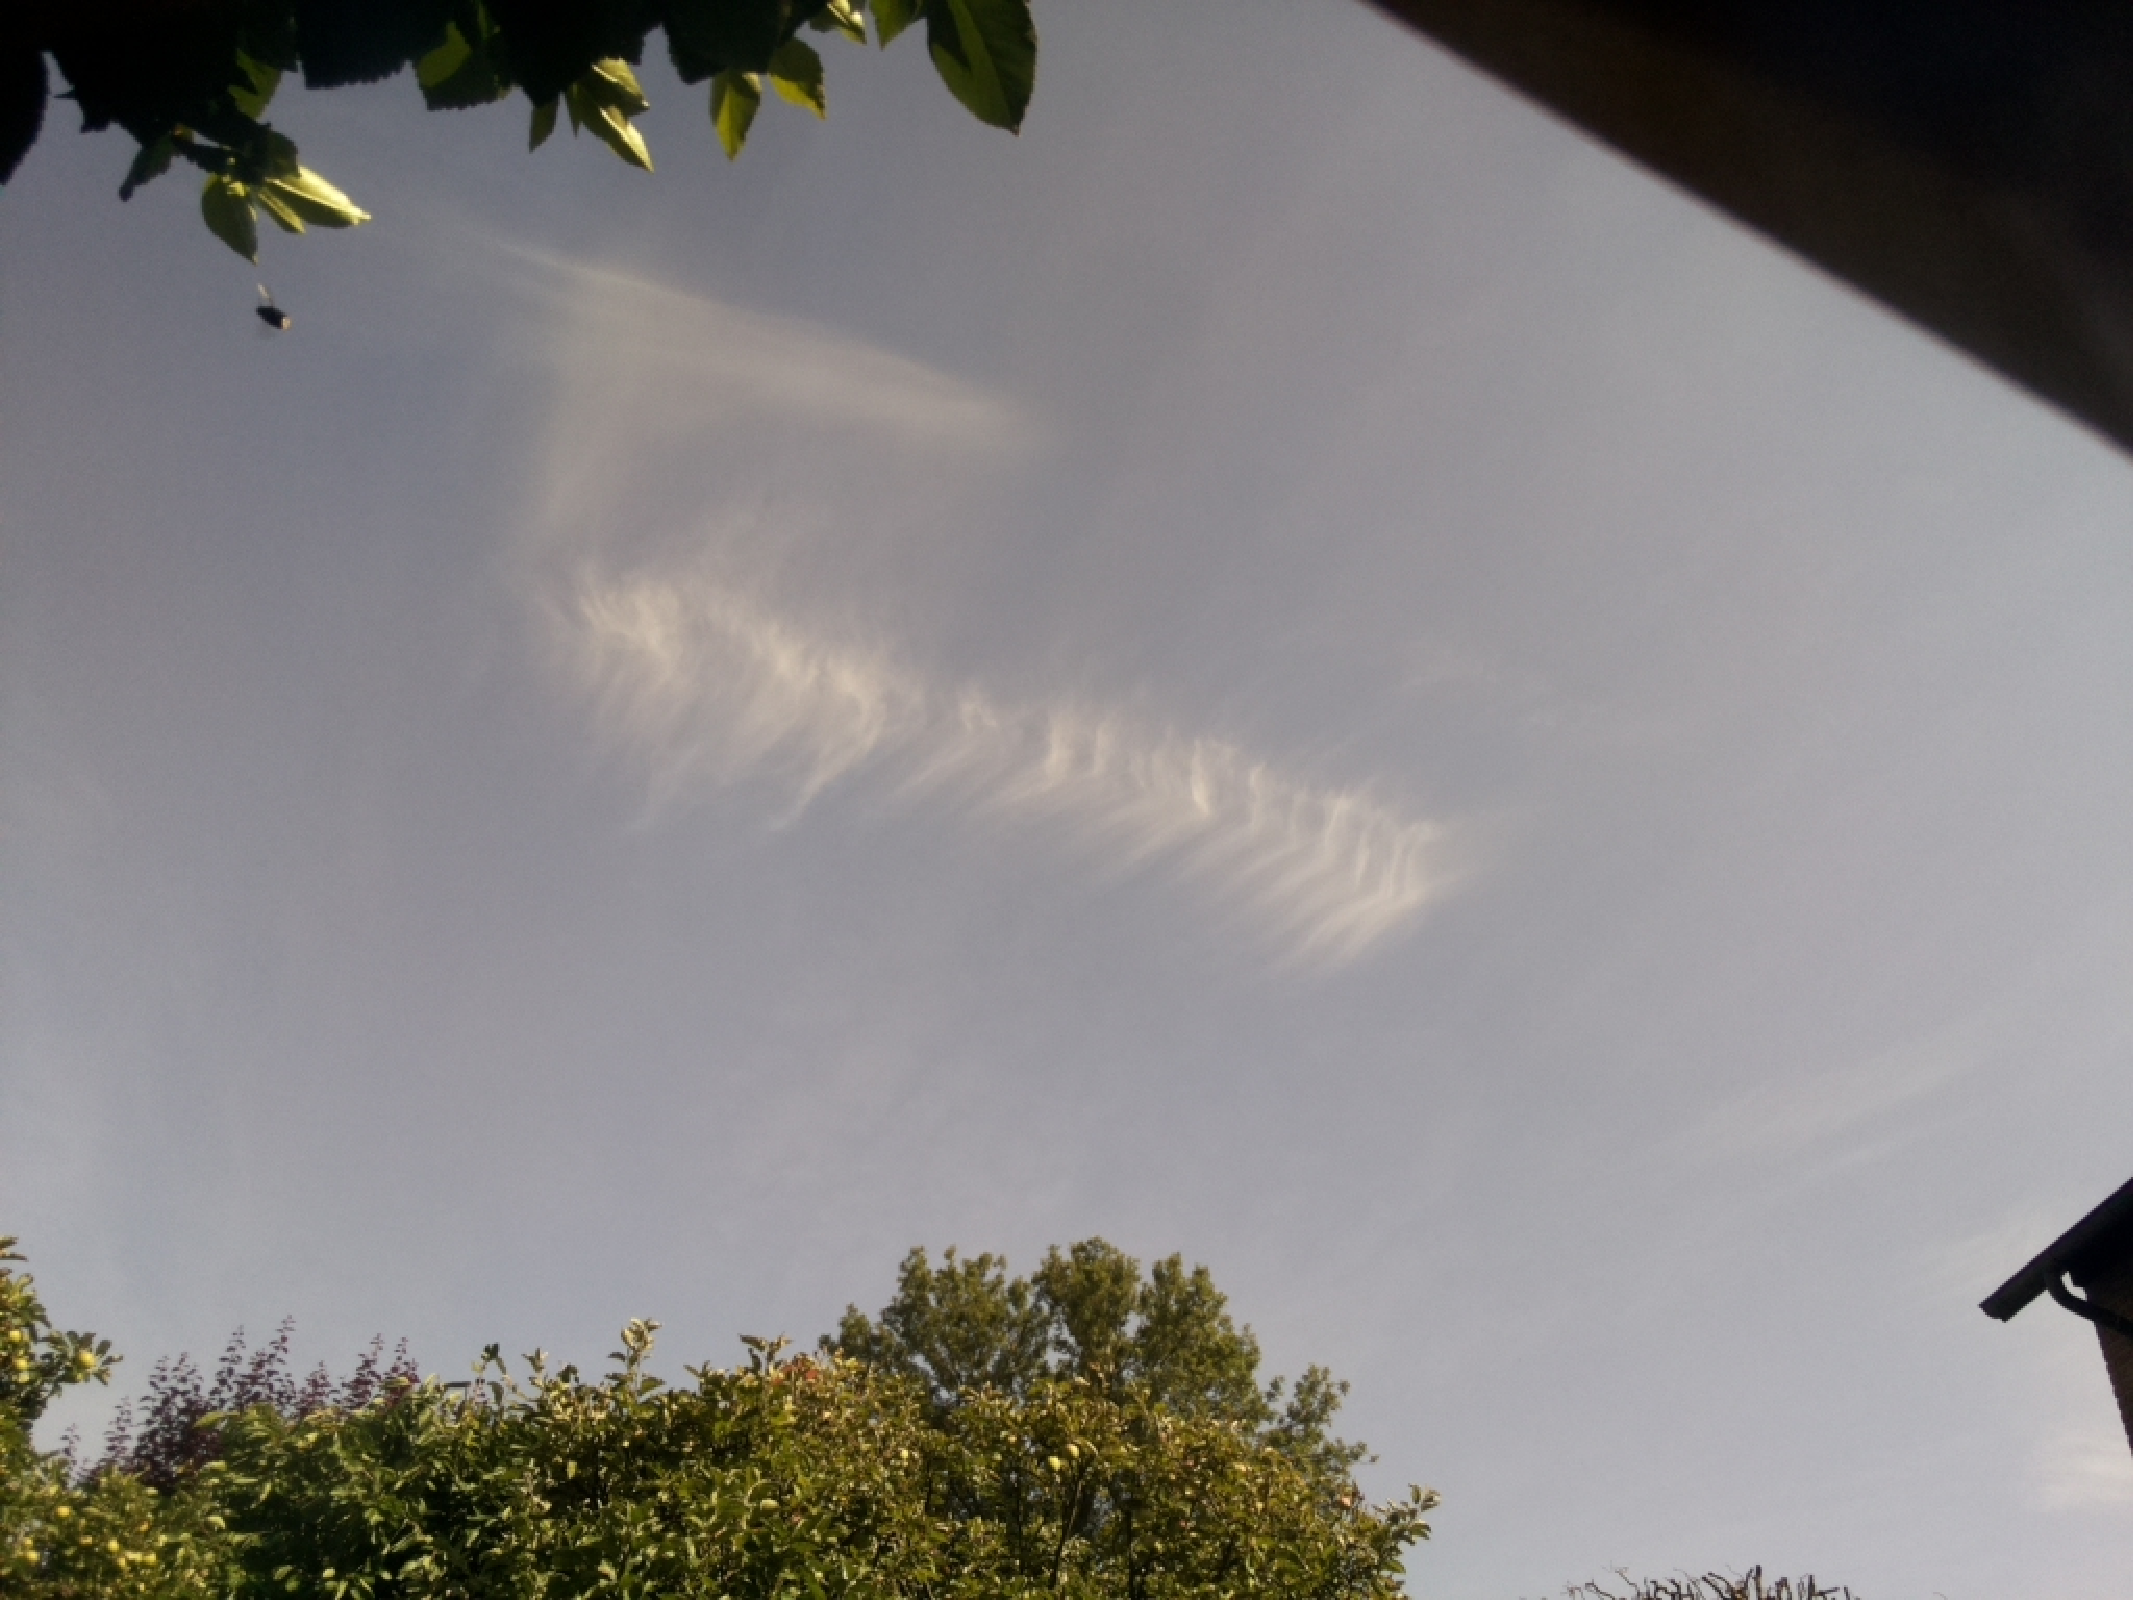
\includegraphics[width=\textwidth]{./pictures/cloudtypes/cirrus.pdf}
		\end{center}
		\caption{Cirrus}
		\label{fig:cirrus}
		\end{subfigure}
		\begin{subfigure}[b]{0.31\textwidth}
		\begin{center}
				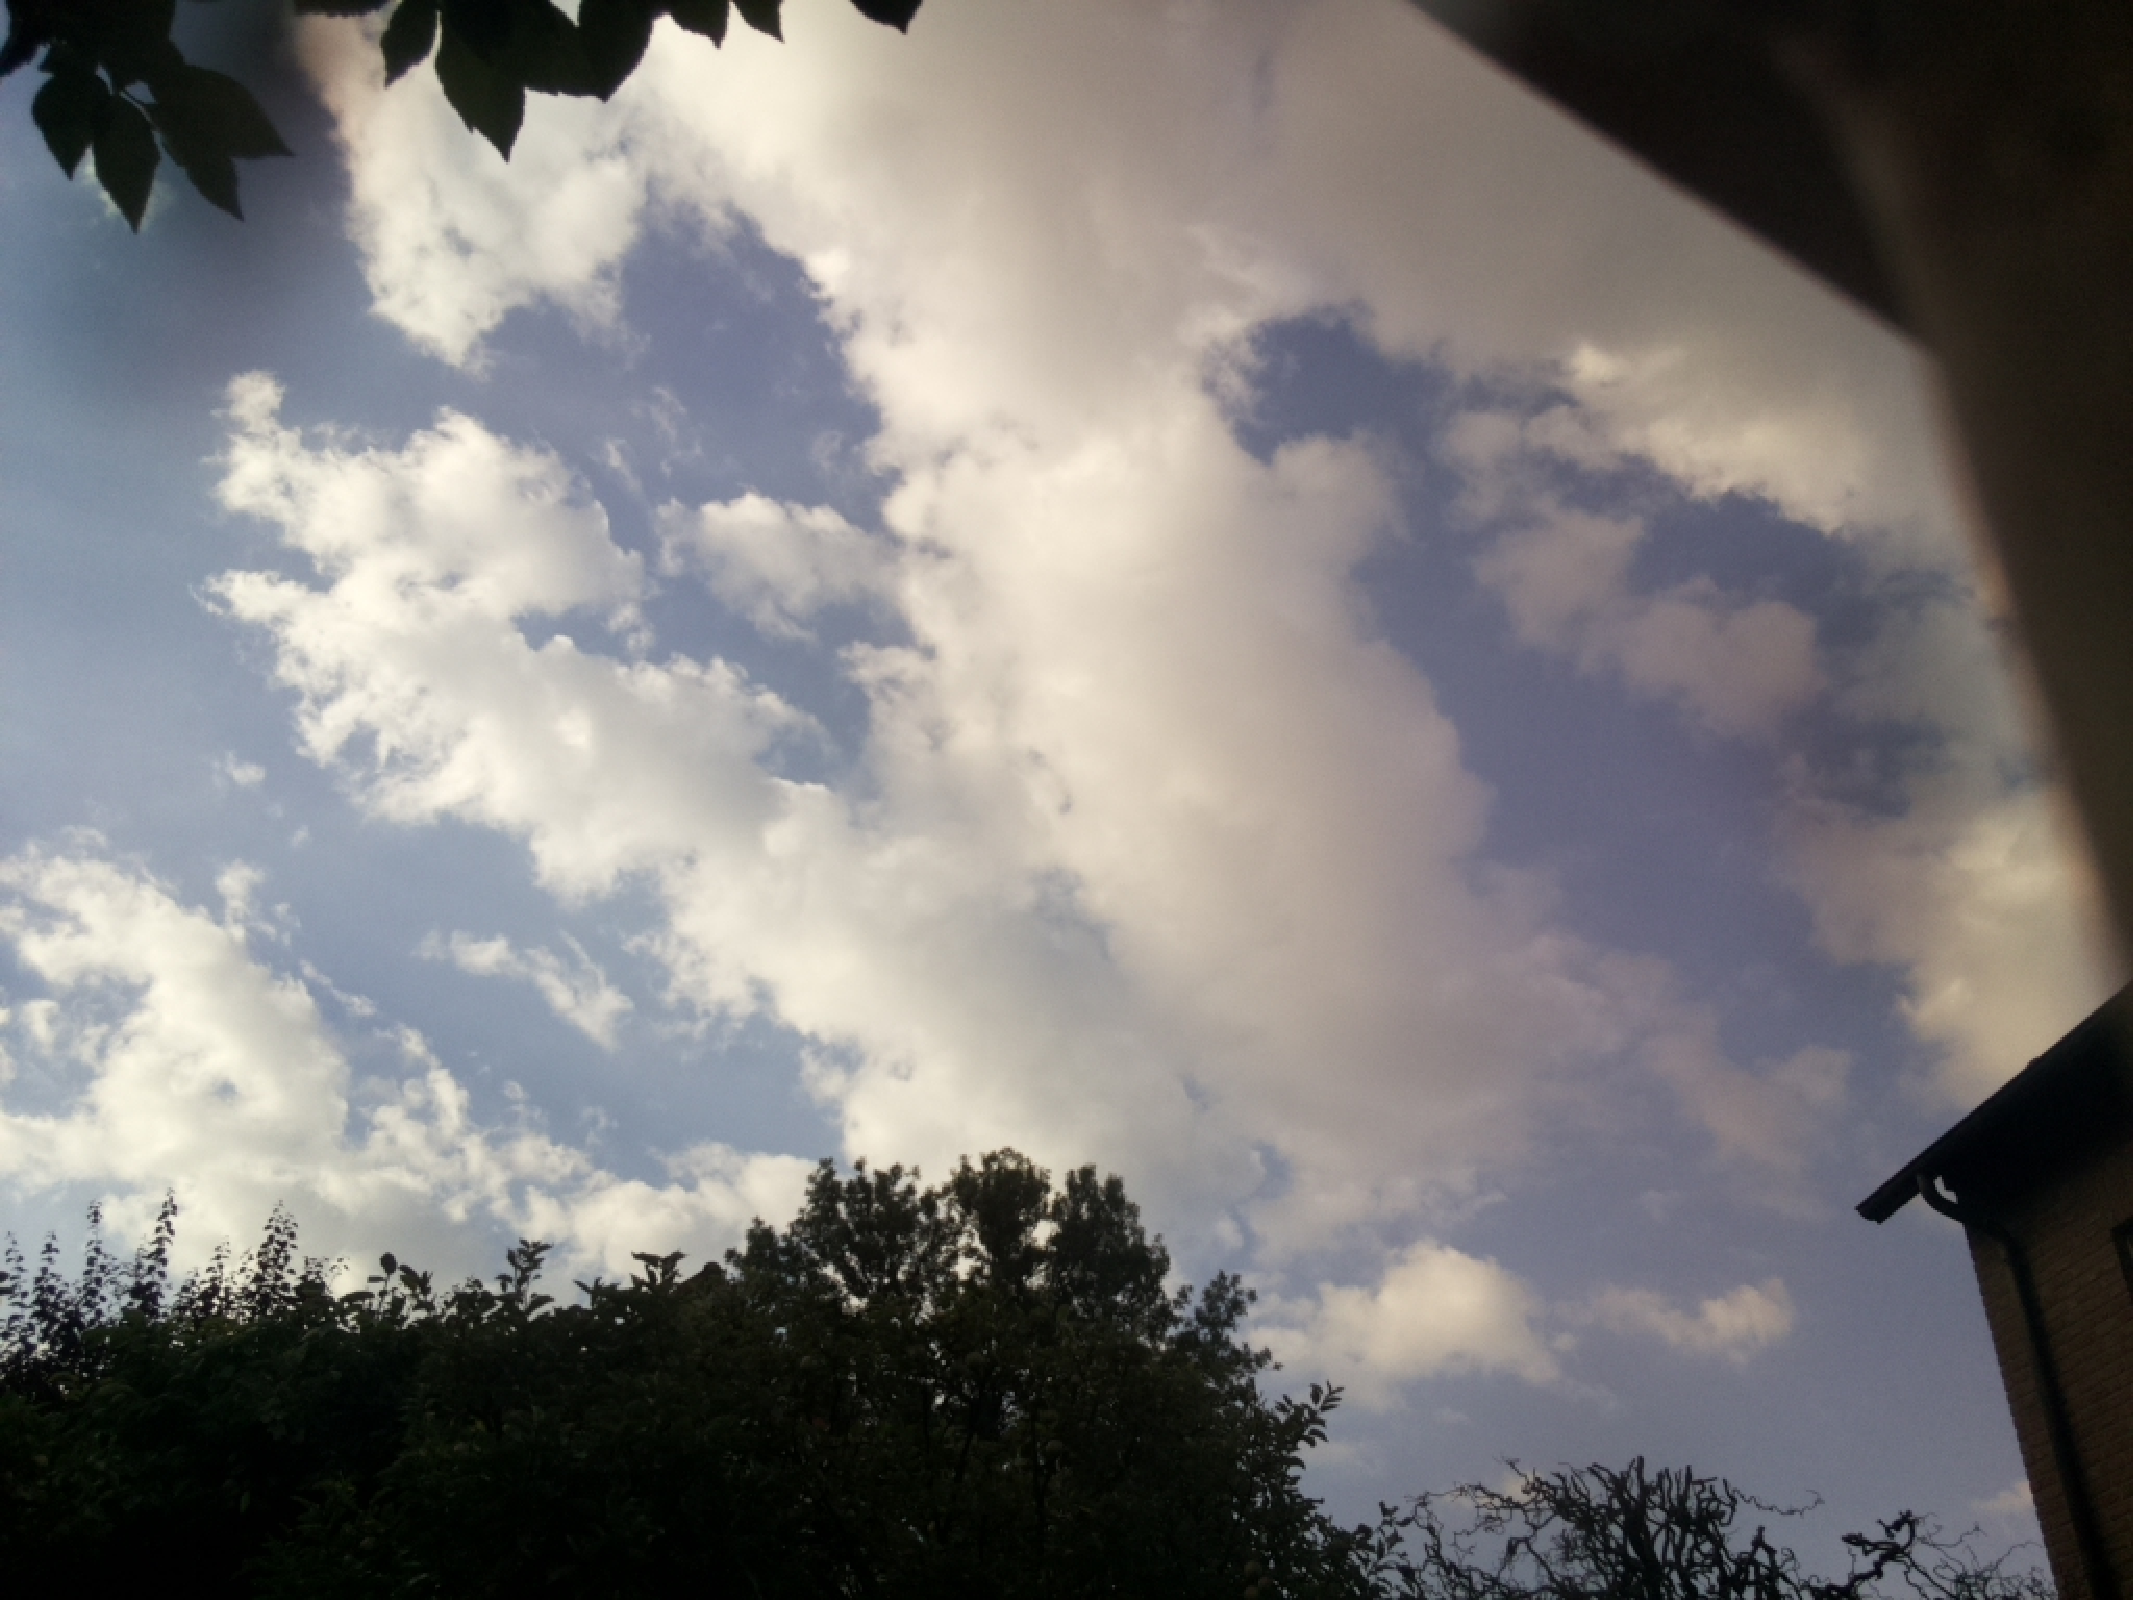
\includegraphics[width=\textwidth]{./pictures/cloudtypes/cumulus.pdf}
		\end{center}
		\caption{Cumulus}
		\label{fig:Cumulus}
		\end{subfigure}
		\begin{subfigure}[b]{0.31\textwidth}
		\begin{center}
				
\includegraphics[width=\textwidth]{./pictures/cloudtypes/nimbostratus.pdf}
		\end{center}
		\caption{Nimbostratus}
		\label{fig:nimbostratus}
		\end{subfigure}
		\begin{subfigure}[b]{0.31\textwidth}
		\begin{center}
				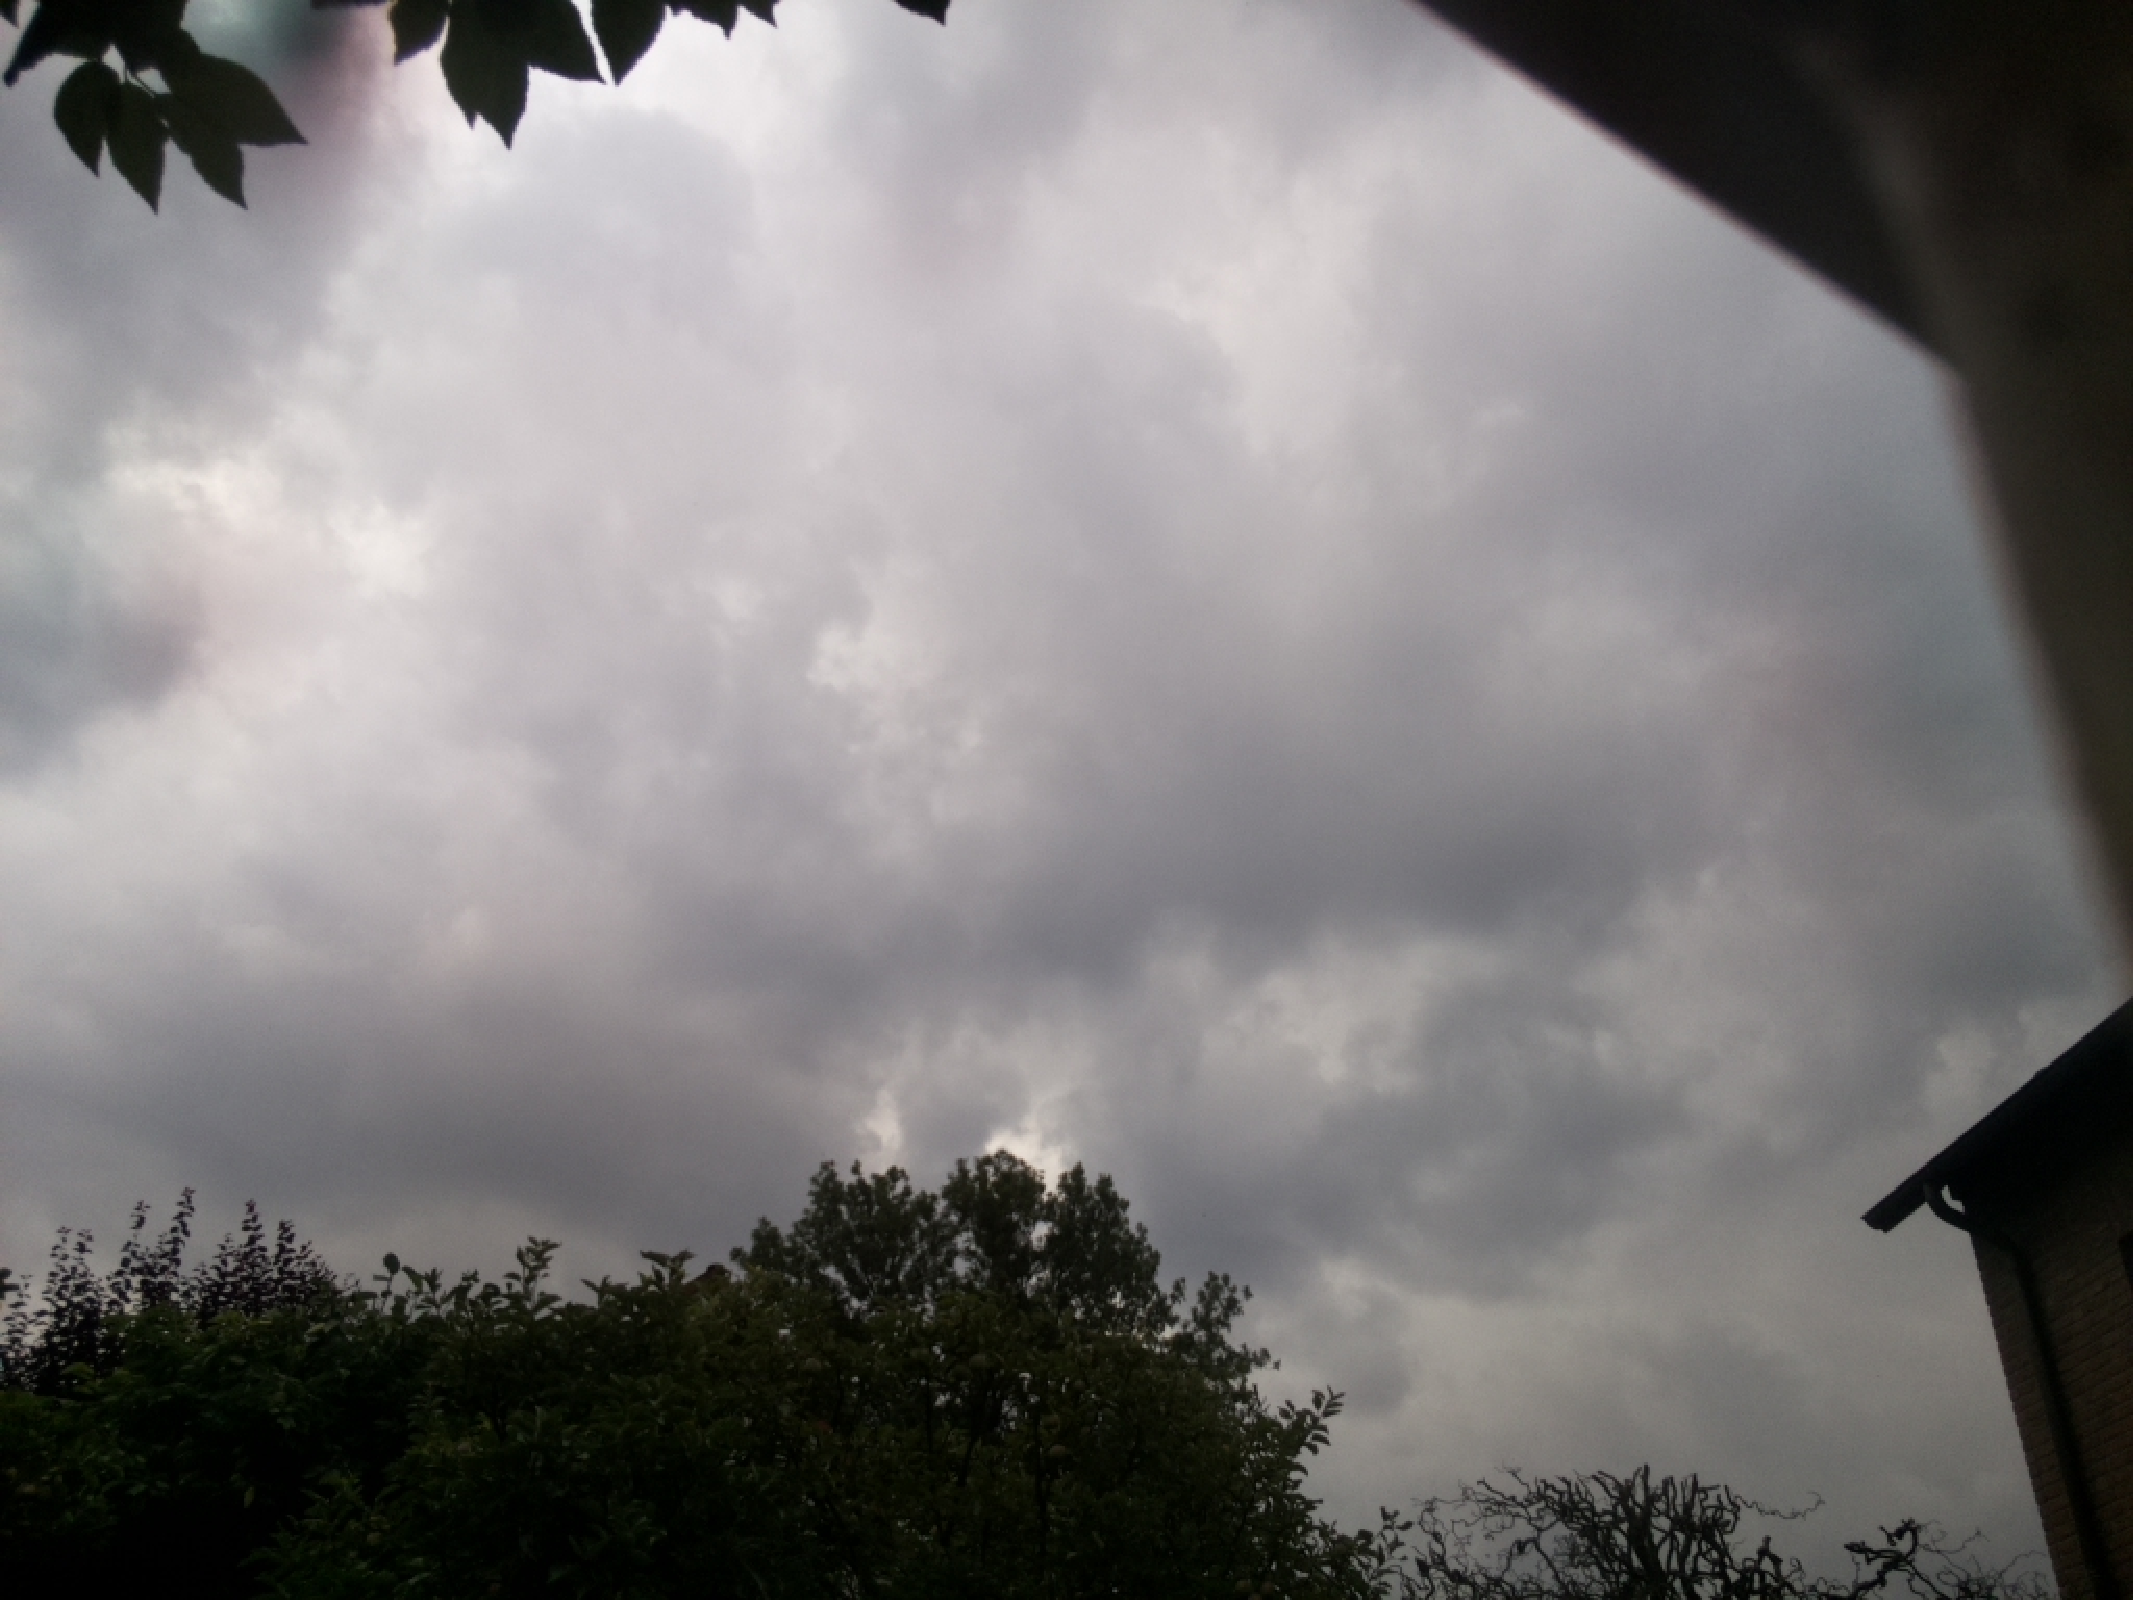
\includegraphics[width=\textwidth]{./pictures/cloudtypes/stratocumulus.pdf}
		\end{center}
		\caption{Stratocumulus}
		\label{fig:stratocumulus}
		\end{subfigure}
		\begin{subfigure}[b]{0.31\textwidth}
		\begin{center}
				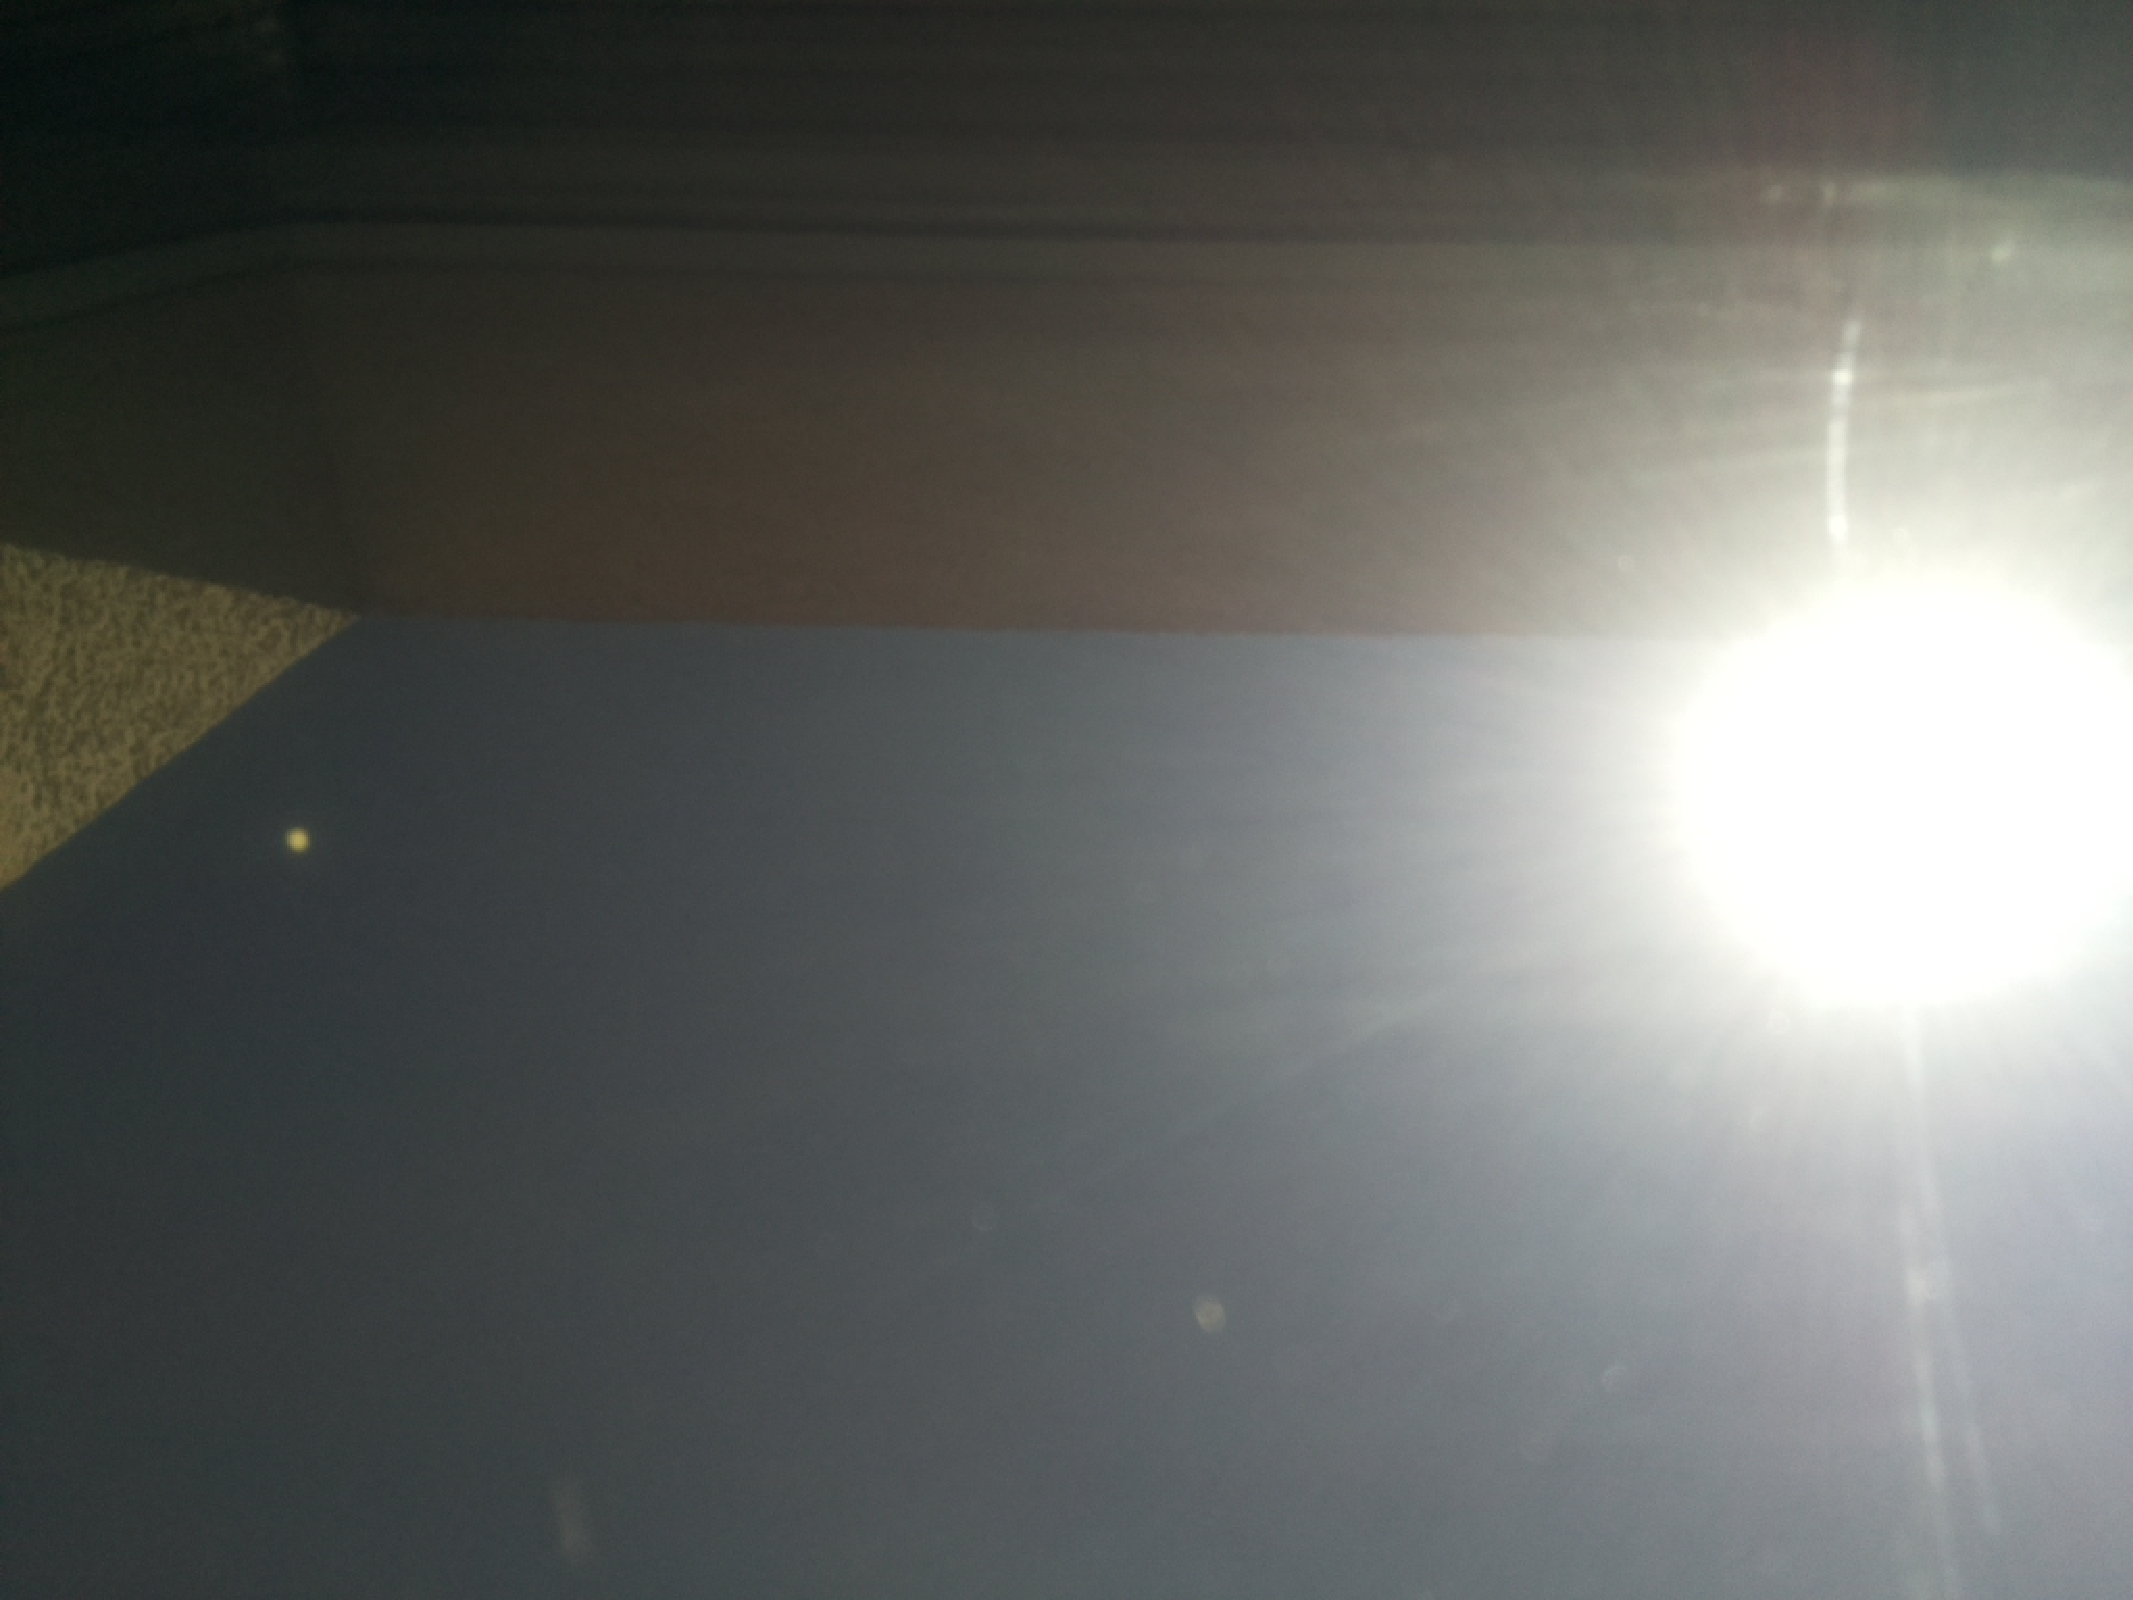
\includegraphics[width=\textwidth]{./pictures/cloudtypes/no_clouds.pdf}
		\end{center}
		\caption{keine Wolken}
		\label{fig:no_clouds}
		\end{subfigure}
		\caption{Repräsentative Fotos für die unterschiedlichen Wolkenklassen.
		Dabei können die Wolkenformen stark variieren. Für umfassendere
		Information können bei dem
		\href{https://telegram.me/weatherpi_bot}{\texttt{TelegramBot}} unter dem
		Punkt \textit{label $\rightarrow$ label $\rightarrow$ info} weitere 
		Informationen angefordert werden.}
		\label{fig:classes}
\end{figure}
